\chapter{多重度、エントロピー、制約付き平衡}

\lectureoverview{確率分布は、その状態がエネルギーを持つと、熱力学的対象となる。まずエントロピーの増大を平衡化と結びつけ、\(dE=T\,dS\)を用いて熱の流れる向きを導く。次に一つの系を多数のレプリカの集まりに置き換え、各占有数の組に対応する配置を数え上げ、この多重度の対数がエントロピーの\(N\)倍であることを示す。したがって平衡は制約付き最大エントロピー問題である。ラグランジュ乗数がそれを解くための方法を与える。}

\section{三つの基本量}

\(i\)が系に許される離散状態を表すものとする。今のところ、離散性は相空間の測度を導入することなく状態を数えられるので有用である。状態\(i\)の確率が\(P_i\)ならば、
\begin{equation}
 \sum_i P_i=1.
 \label{eq:sm3-normalization}
\end{equation}
その状態のエネルギーが\(E_i\)ならば、平均エネルギーは
\begin{equation}
 \overline E=\sum_iP_iE_i.
 \label{eq:sm3-mean-energy}
\end{equation}
\emph{平均}という語が重要である。系が一つの微視的状態において値\(\overline E\)を持つ必要はない。それは可能な値にわたる確率で重み付けした平均である。

\begin{classroomqa}
\classquestion{ここで確率と統計の間に有用な区別はあるか。}
\lecturerresponse{確率は可能な結果の模型を与えるが、統計は通常、観測データから出発し、そこから何が推論できるかを問う。本計算では確率分布を用いるが、同じ平均が統計データにも自然に現れる。授業での非公式なやり取りでは、その区別が続く物理に影響しないため、これらの語は軽く扱われる。
\lecturetimestamp{00:01:39--00:02:21}}
\end{classroomqa}

この分布のエントロピーは
\begin{equation}
 S[P]=-\sum_iP_i\log P_i.
 \label{eq:sm3-entropy}
\end{equation}
この表式は非負である。すべての非零確率は\(0<P_i\leq1\)を満たすので、\(\log P_i\leq0\)であり、\(P_i\to0\)のとき従来の極限値\(P_i\log P_i\to0\)が成り立つ。

\begin{figure}[t]
\centering
\includegraphics[width=0.88\textwidth]{lecture_03_figure_02.png}
\caption{冒頭の板書は、エントロピー、規格化、平均エネルギーの式を、平衡分布の定性的な族とともにまとめている。}
\lectureframe{00:06:44}
\end{figure}

\section{平衡分布の族}

前回の講義は、平衡分布の一パラメータ族を残した。その族を温度でラベル付けしてもよいが、今は平均エネルギー\(\overline E\)でラベル付けする方が有用である。最低可能エネルギーでは、分布は基底状態に集中する。
\[
 P_i=\delta_{i0}.
\]
そのとき状態についての不確かさはなく、\(S=0\)である。平衡分布がより多くのエネルギー準位に広がるにつれて、その平均エネルギーとエントロピーの両方が増大する。

これは熱的な族についての主張であり、考案されうるすべての分布についての主張ではない。任意の族は、より狭くなりながらより大きなエネルギーへ移ることもありうる。導出される平衡分布は、通常の正温度領域ではそのようには振る舞わない。その族に沿って、
\begin{equation}
 \frac{dS}{d\overline E}>0.
 \label{eq:sm3-positive-temperature-branch}
\end{equation}
有界なスペクトルを持つ系は、この導関数が負となる枝を持つこともある。それらの負温度領域は実在するが、本議論では脇に置かれる。

熱平衡は微視的な静止以上のものを意味する。分子は動き、衝突し、エネルギーを交換し続ける。定常になったのは巨視的記述である。分布はもはや正味のドリフトを示さず、系の離れた部分はもはや正味のエネルギー流を支えない。

\section{統計の言葉で表した熱力学法則}

第一法則はエネルギー保存である。第二法則は、孤立した巨視的系の熱力学的エントロピーは減少しないというものである。
\begin{equation}
 \Delta S_{\mathrm{tot}}\geq0.
 \label{eq:sm3-second-law}
\end{equation}
等号は平衡または理想的な可逆変化を表し、自発的な緩和は通常、厳密な増大を与える。

確率的な描像では、緩和は、我々が依然として区別する巨視的な選択肢の上に重みを広げる傾向がある。この主張には講義で強調された限定が必要である。我々は\emph{粗視化}しているのである。厳密なハミルトニアン発展は細視化された相空間エントロピーを保存する。巨視的エントロピーが増大するのは、我々が微視的な相関と詳細を追跡するのをやめるからである。そのような情報を失うことは、縮約された記述を広げる。自発的な狭まりは、代わりに、測定を行うことなく微視的情報を得たことを意味するであろう。

第零法則は、系が熱平衡に達しうること、そして平衡が推移的であることを主張する。\(A\) が \(B\) と平衡にあり、\(B\) が \(C\) と平衡にあるならば、\(A\) は \(C\) と平衡にある。温度は、この推移性を明白にする数を与える：
\[
 T_A=T_B,\qquad T_B=T_C
 \quad\Longrightarrow\quad
 T_A=T_C.
\]
平衡にないとき、エネルギーは温度のより大きい部分系から温度のより小さい部分系へ流れる。温度が等しいとき、正味の流れは止む。次に、この操作的命題を温度のエントロピー定義から導く。

\section{なぜエネルギーは高温から低温へ流れるのか}

弱く結合した二つの部分系 \(A\) と \(B\) を考える。それぞれは内部的に平衡にあるが、それらの温度は異なる。ラベルを
\begin{equation}
 T_B>T_A>0.
 \label{eq:sm3-temperature-order}
\end{equation}
となるように選ぶ。小さな交換の間、合成エネルギーの保存により
\begin{equation}
 dE_A+dE_B=0.
 \label{eq:sm3-energy-conservation}
\end{equation}
が成り立つ。第2法則により
\begin{equation}
 dS_A+dS_B\geq0.
 \label{eq:sm3-entropy-change}
\end{equation}
が成り立つ。内部的に平衡にある各部分系について、温度は
\begin{equation}
 dE_X=T_X\,dS_X,
 \qquad X=A,B.
 \label{eq:sm3-temperature-differential}
\end{equation}
によって定義される。これを \eqref{eq:sm3-energy-conservation} に代入すると
\begin{equation}
 T_A\,dS_A+T_B\,dS_B=0,
\end{equation}
が得られ、したがって
\begin{equation}
 dS_B=-\frac{T_A}{T_B}\,dS_A.
 \label{eq:sm3-dsb}
\end{equation}
となる。この結果を \eqref{eq:sm3-entropy-change} に入れると、
\begin{align}
 dS_{\mathrm{tot}}
 &=dS_A-\frac{T_A}{T_B}dS_A\\
 &=\frac{T_B-T_A}{T_B}\,dS_A\geq0.
 \label{eq:sm3-flow-entropy}
\end{align}
となる。\(T_B-T_A>0\) かつ \(T_B>0\) であるから、自発的な交換には
\[
 dS_A>0.
\]
が必要である。すると式 \eqref{eq:sm3-temperature-differential} により
\begin{equation}
 dE_A=T_A\,dS_A>0,
 \qquad
 dE_B=-dE_A<0.
 \label{eq:sm3-hot-to-cold}
\end{equation}
が得られる。エネルギーは、より高温の部分系である \(B\) から、より低温の \(A\) へ流れた。ここで熱とは、単に移動中のエネルギーである。流れは \(T_A=T_B\) となるまで続き、そのとき一次のエントロピー変化はもはやどちらの向きも有利にしない。

同じ結果は一行で表示できる：
\begin{equation}
 dS_{\mathrm{tot}}
 =dE_A\left(\frac{1}{T_A}-\frac{1}{T_B}\right)\geq0.
 \label{eq:sm3-compact-flow}
\end{equation}
逆温度差の符号が \(dE_A\) の符号を定める。この簡潔な形は、後に正準集団と自然に適合するであろう。

\begin{classroomqa}
\audiencequestion{この議論は、\(A\) と \(B\) がそれぞれすでに内部平衡にあることを仮定しているのか。}
\lecturerresponse{はい。単一の \(T_A\) または \(T_B\) を割り当てることは、その仮定を置くことである。部分系が内部的に平衡でないなら、それをより小さな領域に分割し、温度を定義できるところで局所的にこの議論を適用する。そのとき大域的な緩和は、それらの領域間の交換から組み立てられる。
\lecturetimestamp{00:24:38--00:25:22}}
\end{classroomqa}

\section{何が状態と数えられるのか}

平衡確率を問う前に、ラベル \(i\) が何を意味するのかを知らなければならない。微視的状態とは、基礎となる物理法則によって許される、系の最も完全な指定である。古典力学では、すべての粒子の位置と運動量を思い描く。量子力学では、状態は代わりに完全な量子状態であり、不確定性原理はすべての古典的な位置と運動量を同時に鋭く指定することを妨げる。

有限の箱の中の量子系では、関連する状態の数え上げは離散的でありうる。古典統計力学は適切な極限で現れ、そこでは密に間隔を置いた量子状態にわたる和が相空間積分になる。その極限操作はまた、連続的なエントロピーを無次元にするために必要な相空間セルを導入する。それは単に和の記号を積分の記号に置き換えることによって得られるのではない。

\begin{classroomqa}
\audiencequestion{気体について、状態はすべての分子の位置と運動量として思い描くべきなのか。}
\lecturerresponse{それが正しい古典的描像である。より一般には、状態とは、物理法則に従う限りで原理的に知りうるすべてを意味する。量子力学はその最大限の記述の形を変え、有限体積での数え上げを離散的にする。量子和から古典積分を回復することは、真の極限議論であり、一行の置き換えではない。
\lecturetimestamp{00:25:31--00:27:38}}
\end{classroomqa}

\section{レプリカからなる熱浴}

難しい問いは今や避けられない：平衡が確立した後、何が \(P_i\) を決めるのか。

部分系を非常に大きな熱浴と接触させる。エネルギーは行き来してよいが、熱浴はあまりに多くの自由度をもつため、少量のエネルギーの移動はその温度をほとんど変えない。特に便利な熱浴は、部分系自身の弱く結合した多数のレプリカからなる。一つのレプリカが研究対象の系であり、他のレプリカがその環境を構成する。

この構成はしばしば現実の巨視的系を映し出す。大きなほぼ均質な物体を多数の類似したセルに分割する。各セルは部分系であり、残りのセルがその熱浴として働く。レプリカの総数を \(N\) で表す。教室でのデモンストレーションは9個のレプリカと3つの色付き状態ラベルを用いるが、数え上げはそれらの特定の数に依存しない。

\(n_i\) を状態 \(i\) にあるレプリカの数とする。これらは \emph{占有数} である。可能なエネルギー準位は無限に多くありうるが、有限の全エネルギーでは、非常に高い準位のほとんどは無視できるかゼロの占有をもつ。

第一の制約は単にレプリカの数である：
\begin{equation}
 \sum_i n_i=N.
 \label{eq:sm3-number-constraint}
\end{equation}
第二は全エネルギーである：
\begin{equation}
 \sum_i n_iE_i=N\overline E.
 \label{eq:sm3-total-energy-constraint}
\end{equation}
右辺は示量的である。レプリカの数を2倍にし、その統計的状態を固定したままにすれば、全エネルギーは2倍になるが、レプリカ1個あたりの平均エネルギーは\(\overline E\)のままである。

\begin{classroomqa}
\audiencequestion{レプリカ構成はエネルギー制約も満たさなければならないか。}
\lecturerresponse{はい。占有数は\(N\)に加算されなければならず、そのエネルギー重み付き和は固定された全エネルギー\(N\overline E\)に等しくなければならない。これらはまさに、後にエントロピー最大値を制限することになる二つの制約である。
\lecturetimestamp{00:37:12--00:39:54}}
\end{classroomqa}

無作為に選ばれたレプリカが状態\(i\)を占める確率は、その相対頻度である：
\begin{equation}
 P_i=\frac{n_i}{N},
 \qquad
 n_i=NP_i.
 \label{eq:sm3-frequency-probability}
\end{equation}

\begin{figure}[t]
\centering
\includegraphics[width=0.82\textwidth]{lecture_03_figure_03.png}
\caption{エネルギー準位の描像と、確率を占有分率\(P_i=n_i/N\)と同一視すること。}
\lectureframe{00:41:40}
\end{figure}

\begin{classroomqa}
\audiencequestion{黒板にある\(N(i)\)という記法は\(n_i\)と異なる意味を意図しているのか。}
\lecturerresponse{いいえ。どちらも状態\(i\)の占有数を表す。我々は\(n_i\)を一貫して用い、大文字の\(N\)はレプリカの総数に取ってある。
\lecturetimestamp{00:41:28--00:41:33}}
\end{classroomqa}

\eqref{eq:sm3-number-constraint}と\eqref{eq:sm3-total-energy-constraint}を\(N\)で割ると、確率の制約が再現される：
\begin{equation}
 \sum_iP_i=1,
 \qquad
 \sum_iP_iE_i=\overline E.
 \label{eq:sm3-probability-constraints}
\end{equation}
したがって、アンサンブル頻度の解釈は、我々が出発点とした方程式を再現した。

\section{占有パターンの多重度}

占有数の組\(\{n_i\}\)を固定する。\(N\)個の区別可能なレプリカを状態に割り当てて、ちょうどその組を実現する方法は何通りあるか。答えは多項係数
\begin{equation}
 C(\{n_i\})=\frac{N!}{\prod_i n_i!}.
 \label{eq:sm3-multiplicity}
\end{equation}
である。分母を見るには、まず\(N\)個のラベル付きレプリカを\(N!\)通りに並べる。同じ状態を占める\(n_i\)個のレプリカを入れ替えても新しい占有の割り当ては生じないので、各状態について\(n_i!\)で割る。

\begin{figure}[t]
\centering
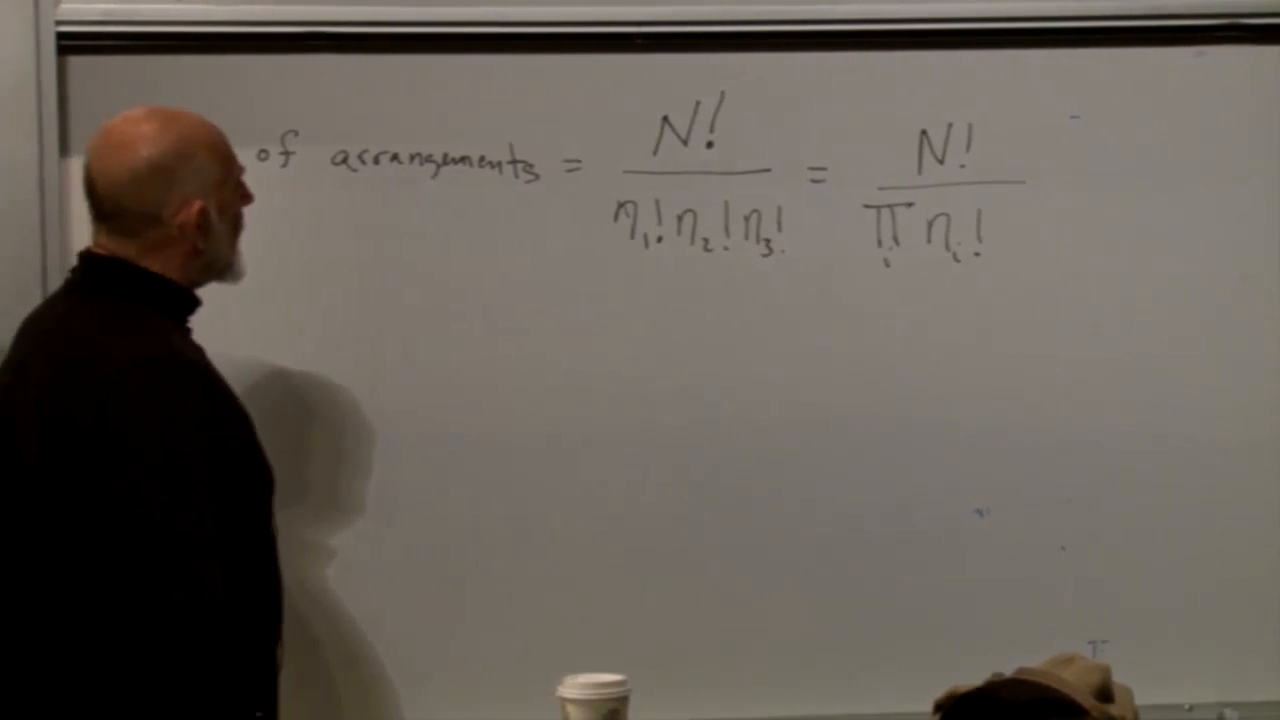
\includegraphics[width=0.88\textwidth]{lecture_03_figure_04.png}
\caption{黒板に書かれた多項係数の多重度\(C=N!/\prod_i n_i!\)。}
\lectureframe{00:46:55}
\end{figure}

占有されていない準位は\(0!=1\)であるから問題を生じない。すべてのレプリカが一つの状態を占めるならば、予想どおり
\[
 C=\frac{N!}{N!}=1,
\]
となる。3個のレプリカが指定された3つの異なる状態を占めるならば、
\[
 C=\frac{3!}{1!\,1!\,1!}=6.
\]
である。2個のレプリカが指定された2つの状態を占める場合、この式は2通りの割り当てを与える：どのラベル付きレプリカがどちらの状態を占めるかを交換するのである。

\begin{classroomqa}
\audiencequestion{二つの制約を満たす占有数の組は複数あり得るか。}
\lecturerresponse{通常は多数ある。式\eqref{eq:sm3-multiplicity}はまず一つの固定された組\(\{n_i\}\)に対する配置を数えるだけで、それが制約を満たすかどうかはまだ決めていない。次の段階では、制約に適合するすべての組を比較し、どれが最大の多重度をもつかを見出す。
\lecturetimestamp{00:48:07--00:48:43}}
\end{classroomqa}

統計的仮定とは、孤立した設定と両立する微視的割り当てを対称に扱うことである。したがって、より多くの割り当てによって実現される巨視的占有パターンの方がより確からしい。大きな\(N\)に対して、分率\(n_i/N\)の上の分布は鋭く尖る。平衡分率は、\eqref{eq:sm3-number-constraint}と\eqref{eq:sm3-total-energy-constraint}を条件として\(C\)を最大化する値である。

\section{スターリングの近似}

階乗は\(N\)が巨視的な値に達するはるか前に巨大になるので、我々はその対数を扱う。まず
\begin{equation}
 \log N!=\sum_{x=1}^{N}\log x.
 \label{eq:sm3-log-factorial-sum}
\end{equation}
から始める。大きな\(N\)に対して、和は\(\log x\)の下の面積で近似される：
\begin{align}
 \log N!
 &\simeq\int_1^N\log x\,dx\\
 &=\left[x\log x-x\right]_1^N\\
 &=N\log N-N+1.
 \label{eq:sm3-stirling-integral}
\end{align}
原始関数は
\[
 \frac{d}{dx}(x\log x-x)=\log x.
\]
から直ちに従う。主要な示量的次数では、加法的定数は落としてよい：
\begin{equation}
 \log N!\simeq N\log N-N.
 \label{eq:sm3-stirling-log}
\end{equation}
指数をとると、講義で用いられた簡略形
\begin{equation}
 N!\simeq N^N e^{-N}.
 \label{eq:sm3-stirling-simple}
\end{equation}
が得られる。

\begin{figure}[t]
\centering
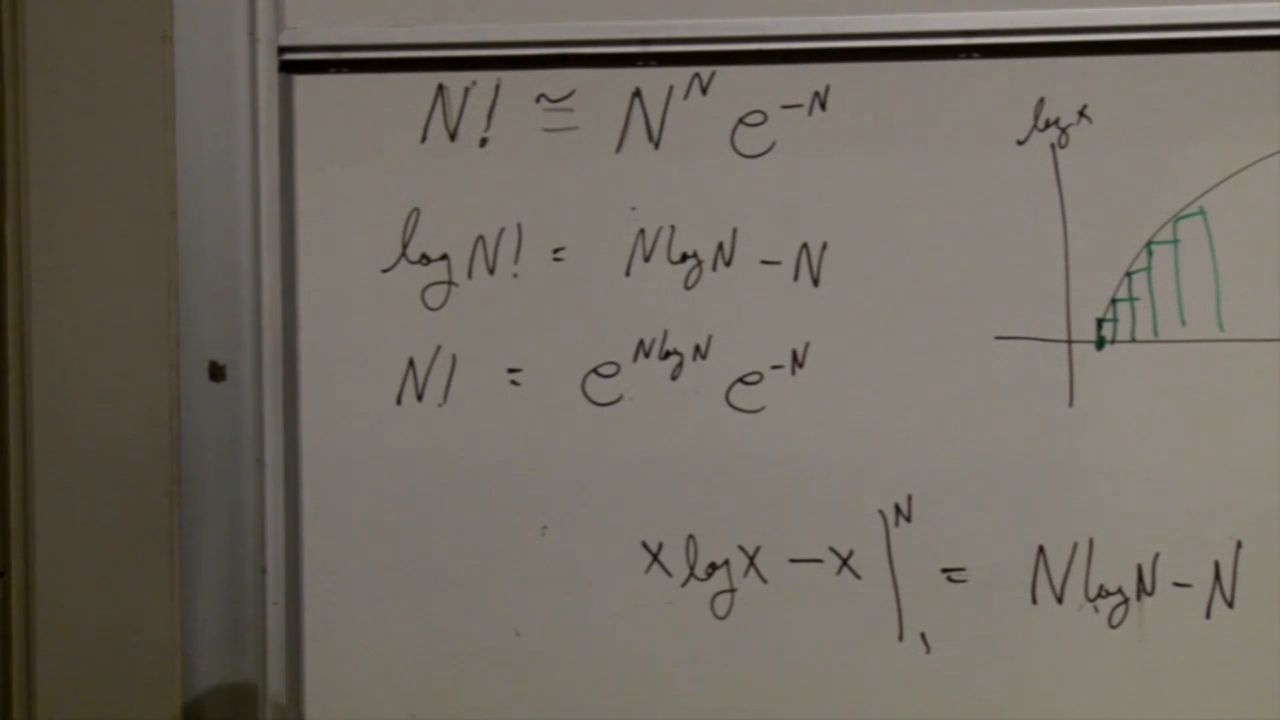
\includegraphics[width=0.88\textwidth]{lecture_03_figure_05.png}
\caption{主要なスターリング近似と、\(\log x\)の和を積分で置き換えることによるその導出。}
\lectureframe{01:03:45}
\end{figure}

\begin{classroomqa}
\audiencequestion{\(x\log x-x\)を下限で評価すると余分な\(+1\)が残るか。}
\lecturerresponse{はい。式\eqref{eq:sm3-stirling-integral}はその定数を含む。\(N\to\infty\)のとき、それは\(N\)に比例する項に比べて無視できる。だから主要な式ではそれを省く。和自体は\(x=1\)から始めなければならない。\(\log0\)は定義されない。
\lecturetimestamp{01:04:12--01:04:35}}
\end{classroomqa}

\begin{classroomqa}
\audiencequestion{\(\sqrt{N}\)に比例する因子も欠けているか。}
\lecturerresponse{はい。より精密な漸近式は
\[
 N!\sim\sqrt{2\pi N}\left(\frac{N}{e}\right)^N.
\]
である。その対数は\(\tfrac12\log(2\pi N)\)だけを加えるが、これは\(N\log N-N\)に比べて非示量的である。それは正確な有限\(N\)の確率には重要だが、巨視的系の主要なエントロピー計算には重要でない。
\lecturetimestamp{01:04:35--01:05:40}}
\end{classroomqa}

スターリングの近似は、\eqref{eq:sm3-multiplicity} の分母においても注意して用いなければならない。熱力学的極限では、ゼロでない極限確率をもつ状態は \(n_i=NP_i\) を満たすので、その占有数は \(N\) とともに増大する。占有数がごく小さいか消えてしまう状態は、有限のエネルギー遮断で扱い、その後で極限をとることによって復元できる。主要な示量的エントロピーは、省略された次次の項によって影響を受けない。

\section{多重度の対数はエントロピーである}

\eqref{eq:sm3-stirling-simple} を分子および巨視的に占有されたすべての分母因子に適用する：
\begin{equation}
 C\simeq
 \frac{N^Ne^{-N}}
 {\prod_i n_i^{\,n_i}e^{-n_i}}.
 \label{eq:sm3-c-stirling}
\end{equation}
\(\sum_i n_i=N\) であるから、主要な指数因子は相殺する：
\begin{equation}
 C\simeq\frac{N^N}{\prod_i n_i^{\,n_i}}.
 \label{eq:sm3-c-leading}
\end{equation}
積よりも対数のほうが最大化しやすく、また対数は単調であるから、両方の極大は同じ占有パターンで起こる：
\begin{equation}
 \log C=N\log N-\sum_i n_i\log n_i.
 \label{eq:sm3-logc-occupations}
\end{equation}
ここで \(n_i=NP_i\) を代入する：
\begin{align}
 \log C
 &=N\log N-\sum_iNP_i\log(NP_i)\\
 &=N\log N-N\sum_iP_i\log N
   -N\sum_iP_i\log P_i\\
 &=-N\sum_iP_i\log P_i,
 \label{eq:sm3-logc-entropy-derivation}
\end{align}
ここで規格化により二つの \(N\log N\) の項が相殺される。したがって、\(N\) の主要な次数まで、
\begin{equation}
 \boxed{\log C=NS}.
 \label{eq:sm3-logc-ns}
\end{equation}

\begin{figure}[t]
\centering
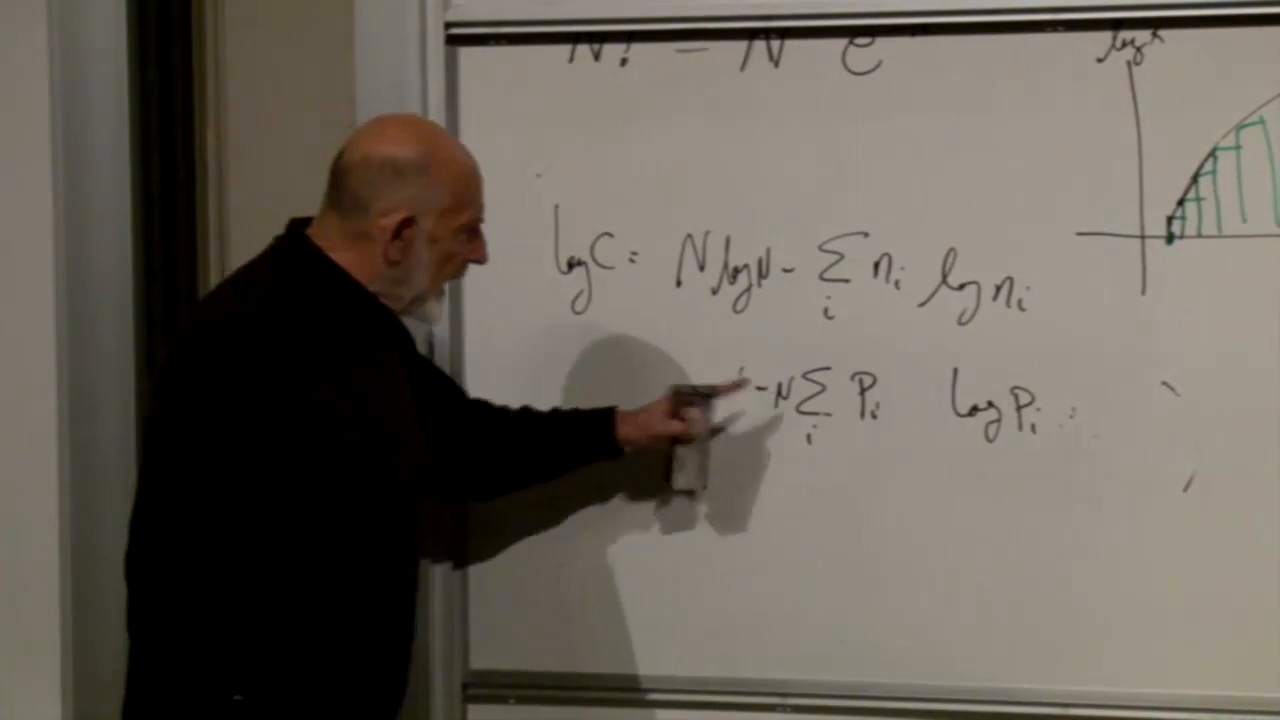
\includegraphics[width=0.88\textwidth]{lecture_03_figure_06.png}
\caption{\(\log C=N\log N-\sum_i n_i\log n_i\) を
\(-N\sum_iP_i\log P_i=NS\) に結びつける板書の計算。}
\lectureframe{01:16:10}
\end{figure}

この関係はこの章の概念的中心である。エントロピーは、数え上げ問題に押しつけられた無関係な量ではない。それは、対数的に測られた、一つのレプリカあたりの多重度である。したがって、微視的配置の数を最大化することは、主要な次数において、一つのレプリカのエントロピーを最大化することと同一である。

\begin{classroomqa}
\audiencequestion{すべての占有数が等しいときに多重度が最大になるのではないか。}
\lecturerresponse{どの状態も区別されず、有限個の状態にわたって \(\sum_i n_i=N\) だけが課されているときには一様である。固定エネルギーの拘束は、値 \(E_i\) が異なるために答えを変える。等しい占有は一般に、指定された平均エネルギーを生み出さない。
\lecturetimestamp{01:17:07--01:18:20}}
\end{classroomqa}

\begin{classroomqa}
\audiencequestion{大文字の \(N\) は大きいが、なぜスターリングの近似を分母のすべての \(n_i\) に適用してよいのか。}
\lecturerresponse{ゼロでない極限確率をもつ各状態について、\(n_i=NP_i\) は \(N\) に比例して増大する。まず有限のエネルギー範囲を保ち、そこで大きな \(N\) の極限をとり、その後で範囲を広げればよい。まばらな裾の状態には別個の有限補正が必要であるが、それらは主要な示量的エントロピーを変えない。
\lecturetimestamp{01:18:23--01:19:28}}
\end{classroomqa}

\begin{classroomqa}
\audiencequestion{この大きな \(N\) の近似が、以前に粗視化によって意味されていたものか。}
\lecturerresponse{いいえ。熱力学的極限は、大きな占有数と漸近的な数え上げを制御する。粗視化は、微視的分解能の喪失または意図的な破棄である。両者はしばしば巨視的統計力学でともに用いられるが、別個の操作である。
\lecturetimestamp{01:19:29--01:19:46}}
\end{classroomqa}

\begin{classroomqa}
\audiencequestion{
\(\log C=N\log N-\sum_i n_i\log n_i\) であるから、第二項は最大化ではなく最小化されるべきではないか。}
\lecturerresponse{はい。\(N\) を固定すると、\(\log C\) を最大化することは \(\sum_i n_i\log n_i\) を最小化することと等価である。\(n_i=NP_i\) を代入した後、固定された \(N\log N\) の項は相殺し、残るのは
\(-N\sum_iP_i\log P_i=NS\) である。したがって、同じ操作は、正のエントロピー \(S\) を最大化することとしてより自然に記述される。
\lecturetimestamp{01:19:48--01:20:55}}
\end{classroomqa}

\begin{classroomqa}
\audiencequestion{なぜ対称性によって直ちに議論を終え、すべての \(n_i\) を等しいと置かないのか。}
\lecturerresponse{その近道はエネルギーのラベルを無視している。規格化の拘束は状態を対称に扱うが、
\(\sum_iP_iE_i=\overline E\) はそうではない。異なるエネルギーの状態は異なる寄与をする。エネルギー拘束こそが、一様でない平衡分布が入ってくるまさにその場所である。
\lecturetimestamp{01:21:15--01:21:41}}
\end{classroomqa}

\section{最大エントロピー問題}

これで統計力学的規則を曖昧さなく述べることができる。確率 \(P_i\) を変化させて、
\begin{equation}
 S[P]=-\sum_iP_i\log P_i
 \label{eq:sm3-maximize-entropy}
\end{equation}
を
\begin{equation}
 \sum_iP_i=1,
 \qquad
 \sum_iP_iE_i=\overline E.
 \label{eq:sm3-maxent-constraints}
\end{equation}
の下で最大化する。最大化する確率は、大きなレプリカ集団の鋭く優先される占有分率を与える。占有数は揺らぐが、その相対的ずれは \(N\) が増大するにつれて縮小するので、比 \(n_i/N\) はよく定義された熱力学的確率となる。

\begin{classroomqa}
\audiencequestion{\(E_i\) は固定された状態エネルギーであり、拘束は別に与えられた全エネルギーを用いるのか。}
\lecturerresponse{はい。スペクトル \(\{E_i\}\) は部分系に属する。完全なレプリカの集まりは固定された全エネルギーをもつが、エネルギーは絶えずレプリカ間を移動する。その全エネルギーを \(N\) で割ることは、一つのレプリカの平均エネルギー \(\overline E\) を固定するのであり、各微視的実現におけるそのエネルギーを固定するのではない。
\lecturetimestamp{01:26:12--01:27:07}}
\end{classroomqa}

問題を述べるのは容易だが、まだ解かれてはいない。二つの拘束をもつ極値化であるから、もう一つの数学的道具が必要である。

\section{ラグランジュ乗数}

制約のない関数 \(F(x_1,x_2,\ldots)\) に対して、停留点は
\begin{equation}
 \frac{\partial F}{\partial x_i}=0
 \qquad\text{for every }i.
 \label{eq:sm3-unconstrained-stationary}
\end{equation}
を満たす。
ここでさらに
\begin{equation}
 G(x_1,x_2,\ldots)=0.
 \label{eq:sm3-one-constraint}
\end{equation}
を要求する。

\begin{classroomqa}
\audiencequestion{図に座標 \(x\) と \(y\) があるとき、\(x\) とは何を意味するのか。}
\lecturerresponse{ここで \(x\) は座標ベクトル全体
\((x_1,x_2,\ldots)\) の略記である。二次元の図では、その成分は単に \(x\) と \(y\) である。後にその成分は確率
\(P_1,P_2,\ldots\) となる。
\lecturetimestamp{01:30:12--01:30:20}}
\end{classroomqa}

幾何学的には、レベル曲線 \(F=\text{constant}\) は等高線図をなし、
一方 \(G=0\) は系が運動を許される曲線である。制約付き極値は、\(F\) のある等高線が制約曲線に接する場所で生じる。その点で勾配は平行である：
\begin{equation}
 \nabla F=-\lambda\nabla G
 \label{eq:sm3-parallel-gradients}
\end{equation}
ある数 \(\lambda\) に対して。

\begin{figure}[t]
\centering
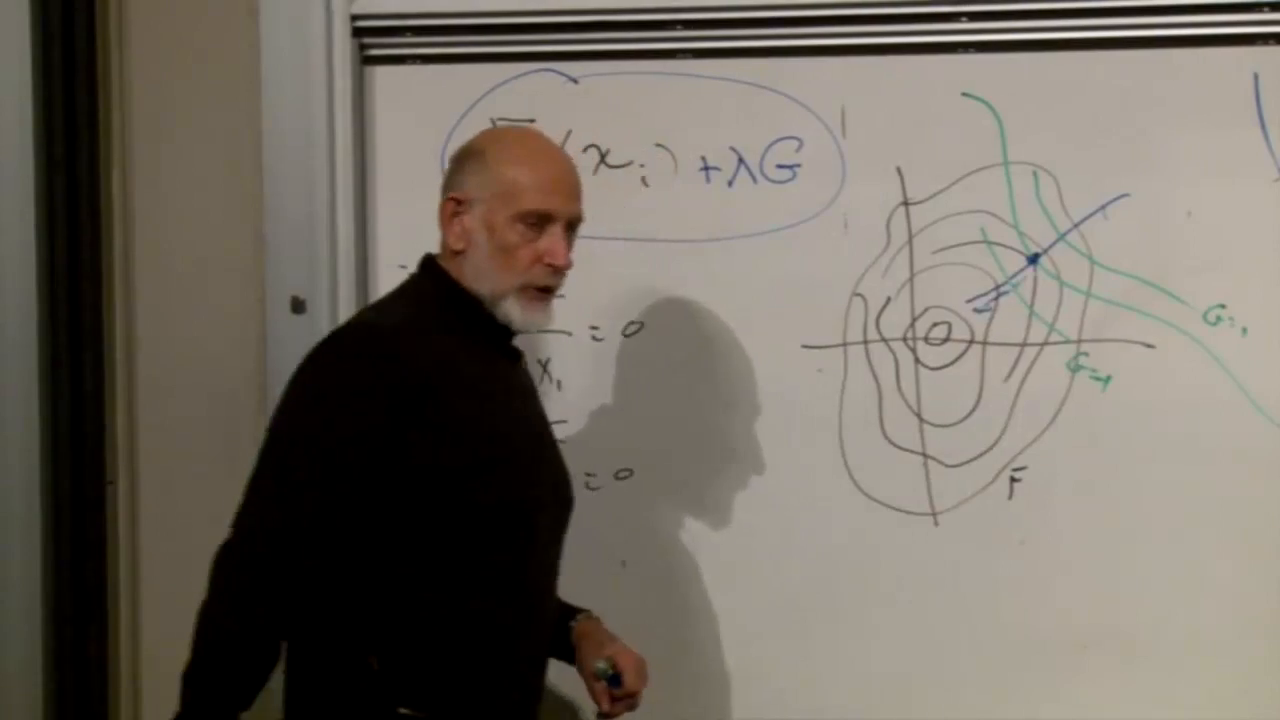
\includegraphics[width=0.88\textwidth]{lecture_03_figure_07.png}
\caption{黒板の等高線幾何と拡張関数
\(F'=F+\lambda G\)。制約付き極値は接点で生じる。}
\lectureframe{01:37:10}
\end{figure}

式 \eqref{eq:sm3-parallel-gradients} は、拡張関数
\begin{equation}
 F'=F+\lambda G
 \label{eq:sm3-augmented-function}
\end{equation}
を定義し、通常の停留性を要求することによって得られる：
\begin{equation}
 \frac{\partial F'}{\partial x_i}=0.
 \label{eq:sm3-augmented-stationarity}
\end{equation}
乗数 \(\lambda\) は最初は未知である。それによって系が不定になるわけではない。なぜなら元の制約 \(G=0\) が追加の方程式を一つ与えるからである。

\begin{classroomqa}
\classquestion{なぜ \(G\) に比例する項を加えると、制約付きの点が停留になるのか。}
\lecturerresponse{制約付き極値では、\(G=0\) に接する方向の運動はすでに \(F\) の一次の変化を生じない。残る傾きは制約に垂直な方向だけである。\(\nabla G\) は同じ垂直方向を向くので、適切な \(\lambda\) がそれを打ち消す：
\(\nabla F+\lambda\nabla G=0\)。
\lecturetimestamp{01:35:06--01:35:32}}
\end{classroomqa}

\section{二変数の例}


\begin{equation}
 F(x,y)=\frac{x^2+y^2}{2}
 \label{eq:sm3-example-f}
\end{equation}
を
\begin{equation}
 x+y=1.
 \label{eq:sm3-example-constraint}
\end{equation}
の下で最小化する。制約を \(G=x+y-1=0\) と書き、
\begin{equation}
 F'=\frac{x^2+y^2}{2}+\lambda(x+y-1).
 \label{eq:sm3-example-augmented}
\end{equation}
を作る。停留方程式は
\begin{align}
 \frac{\partial F'}{\partial x}&=x+\lambda=0,\\
 \frac{\partial F'}{\partial y}&=y+\lambda=0.
 \label{eq:sm3-example-derivatives}
\end{align}
である。したがって \(x=y=-\lambda\)。残る方程式は制約であり、
\[
 x+y=-2\lambda=1,
\]
よって
\begin{equation}
 \lambda=-\frac12,
 \qquad
 x=y=\frac12.
 \label{eq:sm3-example-solution}
\end{equation}
点 \((1/2,1/2)\) は、原点を中心とする最小の円が直線 \(x+y=1\) に接する点である。

\begin{figure}[t]
\centering
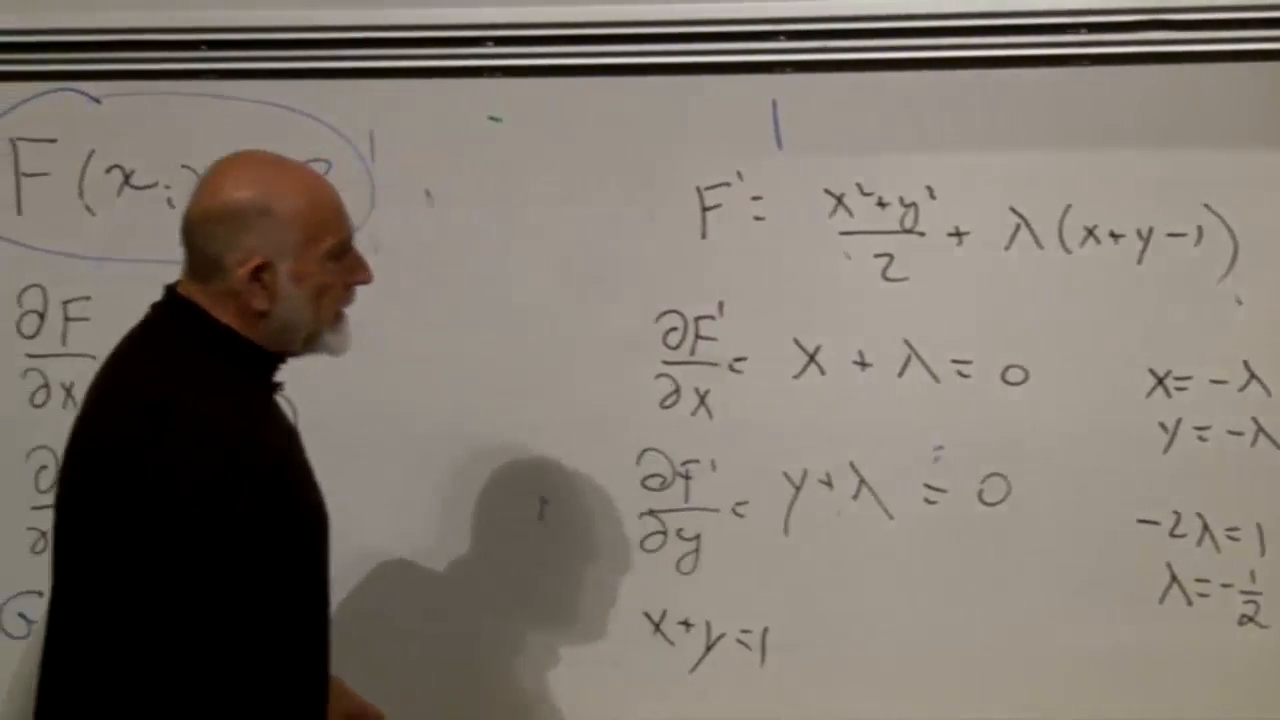
\includegraphics[width=0.88\textwidth]{lecture_03_figure_08.png}
\caption{\(x+y=1\) の下で \((x^2+y^2)/2\) を最小化するための、完成したラグランジュ乗数の計算。}
\lectureframe{01:44:10}
\end{figure}

制約が複数ある場合は、それぞれに一つの乗数を導入する：
\begin{equation}
 F'=F+\lambda_1G_1+\lambda_2G_2+\cdots.
 \label{eq:sm3-many-multipliers}
\end{equation}
次に
\begin{equation}
 \begin{aligned}
 \frac{\partial F'}{\partial x_i}&=0
 &&\text{for every }i,\\
 G_a&=0
 &&\text{for every constraint }a.
 \end{aligned}
 \label{eq:sm3-many-equations}
\end{equation}
を解く。講義では、意図的に人為的な練習問題を提案する：\(x,y,z\) の二次関数を、\(x+y=1\) や \(z+x=1\) のような二つの独立な線形制約を課しながら極値化する。その目的は特定の答えではなく、各制約が一つの乗数と一つの方程式の両方をもたらすという規則である。

\section{次の講義に備えた問題}

統計力学では、座標は確率
\(\{P_i\}\) であり、最大化すべき関数はエントロピーであり、制約は規格化と固定された平均エネルギーである。
\begin{align}
 S[P]&=-\sum_iP_i\log P_i,\\
 G_1[P]&=\sum_iP_i-1,\\
 G_2[P]&=\sum_iP_iE_i-\overline E.
 \label{eq:sm3-final-functions}
\end{align}
を定義する。したがって拡張エントロピーは
\begin{equation}
 \Phi[P]
 =S[P]+\alpha G_1[P]+\beta G_2[P].
 \label{eq:sm3-final-augmented}
\end{equation}
と書ける。解くべき方程式は
\begin{equation}
 \frac{\partial\Phi}{\partial P_i}=0
 \quad\text{for every }i,
 \qquad
 G_1=0,
 \qquad
 G_2=0.
 \label{eq:sm3-final-problem}
\end{equation}

\begin{figure}[H]
\centering
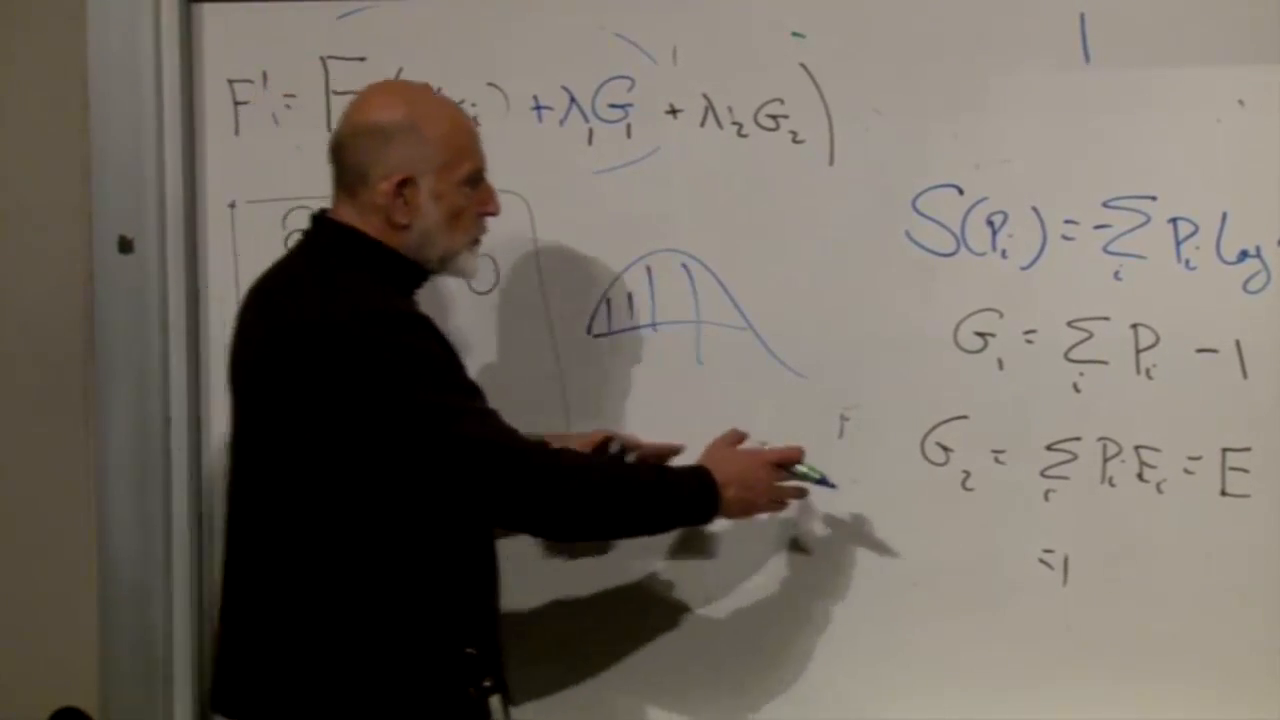
\includegraphics[width=0.88\textwidth]{lecture_03_figure_09.png}
\caption{締めくくりの黒板：確率の関数としてのエントロピー、および規格化と固定された平均エネルギー。}
\lectureframe{01:53:05}
\end{figure}

この時点で問題は完全に定式化された。
\eqref{eq:sm3-final-problem}
を解くと平衡分布が得られる。エネルギーに共役な乗数は、\eqref{eq:sm3-final-augmented} で選ばれた符号の規約を除いて、逆温度
\(\beta=1/T\) となる。次の講義ではその微分を実行し、ボルツマン重みを得る。